\chapter{Modellazione del gioco del 15 con Answer Set Programming (ASP)}
\label{asp}

\section{Introduzione ad ASP \cite{12}}
L'Answer Set Programming (ASP) è un paradigma di programmazione dichiarativa basato sulla programmazione logica, adatto per la risoluzione di problemi di ricerca combinatoria e ragionamento automatico. A differenza della programmazione imperativa tradizionale, dove si specifica come risolvere un problema attraverso una sequenza di istruzioni, in ASP si descrive cosa costituisce una soluzione valida del problema.
Il cuore di ASP risiede nel concetto di "answer set":\\
dato un programma logico, \textbf{un answer set è un insieme di atomi che soddisfa tutte le regole del programma in modo coerente e minimale}. \\
Il sistema ASP trova automaticamente tutti gli answer set possibili, che rappresentano le soluzioni del problema modellato.

\section{Struttura e sintassi}
In \textbf{ASP} (Answer Set Programming), i programmi sono rappresentati come un insieme finito di \textit{regole} della forma: ~\cite{11} \\
$a \leftarrow b_1, \dots, b_m, \text{not } c_1, \dots, \text{not }c_k$ \\
dove:
\begin{itemize}
    \item $a$ è la \textit{testa della regola}
    \item $b_i$, $c_j$ sono \textit{atomi} della logica del primo ordine presenti nel \textit{corpo della regola};
\end{itemize} 

In ASP questo viene rappresentato come: ~\cite{12}

\begin{verbatim}
    <testa> :- <corpo>. 
\end{verbatim}

dove: 
\begin{itemize}
    \item testa è un \textbf{atomo}, cioè una formula atomica ovvero un’espressione che non può essere scomposta ulteriormente usando connettivi logici;
    \item corpo è una \textbf{congiunzione} di letterali ovvero atomi positivi o negativi; 
    \item $:-$ il simbolo indica un "if"; 
\end{itemize}

Le regole in ASP possono assumere diverse forme.

L’atomo nella testa risulta vero se tutti gli atomi positivi nel corpo possono essere derivati e nessuno degli atomi negati (\textit{not} $c_j$) lo può essere, in questo caso la regola prende il nome di \textbf{fatto}.

Le \textit{regole con testa vuota} rappresentano \textbf{vincoli di integrità}, utilizzati per esprimere condizioni di incompatibilità (ad esempio: due componenti che non possono coesistere).

Al contrario, una \textit{regola con corpo vuoto} rappresenta un \textbf{fatto}, cioè un'informazione assunta come vera.

ASP permette anche la definizione di \textit{vincoli di cardinalità}, che specificano scelte tra insiemi di atomi, come `scegliere da 1 a 2 CPU da un insieme disponibile', queste regole prendono il nome di \textbf{regole di scelta}.

La risoluzione di un programma ASP avviene in due fasi: ~\cite{13}
\begin{itemize}
    \item prima il programma viene \textit{groundato}, ovvero tutte le variabili vengono sostituite con costanti dell’universo di Herbrand;
    \item poi il programma senza variabili viene analizzato da un \textit{risolutore ASP}, che calcola i \textit{modelli stabili} (o \textit{answer sets}), ossia le possibili soluzioni minimali che soddisfano tutte le regole.
\end{itemize}

\section{Modellazione del contesto di lavoro a ASP}
Per rappresentare il problema del gioco del 15 e trovare una sequenza minima di mosse per passare da una configurazione iniziale a una finale, utilizziamo \emph{Answer Set Programming} (ASP).

Il modello ASP definisce un dominio temporale discreto, rappresentato dal predicato
\texttt{tempo(0..t)}, dove \( t \) è il massimo numero di mosse ammesse. 
La griglia \(4 \times 4\) è modellata mediante il dominio delle coordinate \texttt{range(0..3)}.

Ogni stato del puzzle è descritto da fatti del tipo \texttt{cell(T,X,Y,V)}, che indicano che al tempo \( T \) la tessera \( V \) si trova nella cella con coordinate \((X,Y)\). La tessera vuota è rappresentata dal valore \(0\).

Lo stato iniziale viene definito assegnando i fatti \texttt{cell(0,X,Y,V)} corrispondenti alla configurazione di partenza. Lo stato obiettivo è codificato come un vincolo che richiede che, al tempo finale \( t \), la disposizione delle tessere corrisponda a quella della configurazione risolta. \\

Le mosse legali sono rappresentate da atomi \texttt{move(T,Dir)}, dove \( Dir \in \{\texttt{up}, \texttt{down}, \texttt{left}, \texttt{right}\} \) indica la direzione dello spostamento del buco nella mossa eseguita al tempo \( T \). Il modello impone che per ogni \( T \) venga eseguita al massimo una mossa e che questa sia valida, ovvero che lo spostamento non esca dalla griglia.

Le regole ASP definiscono la transizione di stato conseguente alla mossa, aggiornando la posizione del buco e delle tessere coinvolte, mentre le celle non modificate mantengono il loro valore per inerzia.

Infine, includiamo una direttiva di minimizzazione.
Questo consente al solver ASP di trovare una soluzione con il numero minimo di mosse necessarie per risolvere il puzzle.

Qui vengono definiti i domini fondamentali del problema. La costante `t=50` stabilisce il numero massimo di mosse consentite. Il predicato `tempo(0..t)` crea il dominio temporale, `val(0..15)` definisce i possibili valori delle tessere (0-15, dove 0 rappresenta il buco), e `range(0..3)` stabilisce le coordinate della griglia 4x4.

\begin{verbatim}
% Parametri
t=50.
tempo(0..t).
range(0..3).
\end{verbatim}

Le seguenti righe di codice definiscono la struttura del predicato principale `cell` che rappresenta lo stato completo del puzzle. Ogni fatto $cell(T,X,Y,V)$ indica che al tempo T, la cella nella riga X e colonna Y contiene il valore V.
Di conseguenza viene definita una configurazione "iniziale" di partenza da cui il gioco inizia.

\begin{verbatim}
% Stato iniziale (esempio)
cell(0,0,0,0). cell(0,0,1,1). cell(0,0,2,7). cell(0,0,3,3).
cell(0,1,0,2). cell(0,1,1,6). cell(0,1,2,8). cell(0,1,3,4).
cell(0,2,0,5). cell(0,2,1,9). cell(0,2,2,11). cell(0,2,3,12).
cell(0,3,0,13). cell(0,3,1,10). cell(0,3,2,14). cell(0,3,3,15).

\end{verbatim}

Allo stesso modo definiamo la configurazione finale del puzzle. Le prime due regole calcolano i valori corretti per ciascuna posizione usando la formula $4*X+Y+1$, che produce la sequenza $1,2,3,4,5,6,7,8,9,10,11,12,13,14,15$. La terza regola specifica che il buco (valore $0$) deve trovarsi nell'angolo in basso a destra. L'ultimo vincolo garantisce che tutte le posizioni soddisfino il goal.

\begin{verbatim}
% Stato finale desiderato
goal(X,Y) :- range(X), range(Y), X < 3, cell(t,X,Y,4*X+Y+1).
goal(X,Y) :- range(X), range(Y), X = 3, Y < 3, cell(t,X,Y,4*X+Y+1).
goal(3,3) :- cell(t,3,3,0).
:- range(X),range(Y), not goal(X,Y).
\end{verbatim}

Questa regola di scelta garantisce che ad ogni istante temporale T venga selezionata esattamente una mossa tra le quattro possibili direzioni (su, giù, sinistra, destra).

\begin{verbatim}
% Una mossa per tempo
1 { move(T,up); move(T,down); move(T,left); move(T,right) } 1 :- tempo(T), T < t.
\end{verbatim}

Questa regola identifica la posizione del buco (tessera vuota con valore 0) al tempo T, informazione necessaria per determinare quali mosse sono possibili.

\begin{verbatim}
hole(T,X,Y) :- cell(T,X,Y,0), tempo(T), range(X), range(Y).
\end{verbatim}

Questi vincoli di integrità impediscono mosse illegali che porterebbero il buco fuori dai confini della griglia. Rispettivamente: non si può muovere su dalla riga 0, non si può muovere giù dalla riga 3, non si può muovere a sinistra dalla colonna 0, e non si può muovere a destra dalla colonna 3.

\begin{verbatim}
%mosse proibite
:- tempo(T), move(T,up),    range(Y), hole(T,0,Y). 
:- tempo(T), move(T,down),  range(Y), hole(T,3,Y). 
:- tempo(T), move(T,left),  range(X), hole(T,X,0). 
:- tempo(T), move(T,right), range(X), hole(T,X,3).
\end{verbatim}

Queste regole determinano quale tessera viene spostata in base alla direzione del movimento del buco. Quando il buco si muove in una direzione, la tessera nella direzione opposta viene spostata nella posizione del buco.

\begin{verbatim}
% Effetti
moved(T,X-1,Y) :-  hole(T,X,Y), move(T,up),    tempo(T),  range(X), range(Y).
moved(T,X+1,Y) :-  hole(T,X,Y), move(T,down),  tempo(T),  range(X), range(Y).
moved(T,X,Y-1) :-  hole(T,X,Y), move(T,left),  tempo(T),  range(X), range(Y).
moved(T,X,Y+1) :-  hole(T,X,Y), move(T,right), tempo(T),  range(X), range(Y).
\end{verbatim}

Questo blocco implementa la transizione di stato. La prima regola stabilisce che la posizione della tessera spostata diventa il nuovo buco (valore 0). La seconda regola sposta il valore della tessera che era nella posizione spostata alla vecchia posizione del buco.

\begin{verbatim}
cell(T+1,X,Y,0)     :-  
     moved(T,X,Y), tempo(T), tempo(T+1), range(X), range(Y). 
cell(T+1,X1,Y1,V)   :-  
    hole(T,X1,Y1), moved(T,X2,Y2), cell(T,X2,Y2,V), 
    tempo(T), tempo(T+1), range(X1), range(X2), range(Y1), range(Y2), val(V).
\end{verbatim}

Questo meccanismo implementa il principio di inerzia: le posizioni non coinvolte nella mossa (né il buco né la tessera spostata) mantengono il loro valore invariato nel tempo successivo.

\begin{verbatim}
% Inerzia
affected(T,X,Y) :- hole(T,X,Y),  tempo(T),  range(X), range(Y).
affected(T,X,Y) :- moved(T,X,Y), tempo(T),  range(X), range(Y).
\end{verbatim}sono le celle che non sono state spostate, in sostanza, perché valga cell(T+1,X,Y,V) devono valere le tre cose dopo.

\begin{verbatim}
cell(T+1,X,Y,V) :-  cell(T,X,Y,V),
       not affected(T,X,Y), 
       tempo(T), tempo(T+1), range(X), range(Y), val(V).
\end{verbatim}

La direttiva "show" specifica che nell'output devono essere mostrate solo le mosse eseguite. La direttiva 'minimize' ottimizza la soluzione cercando di minimizzare il numero totale di mosse necessarie per risolvere il puzzle.

\begin{verbatim}
#show move/2.
#minimize{1,T : move(T,_)}.
\end{verbatim}

\section{Risultati}
Consideriamo una prova con 3 configurazioni del gioco del 15.

\begin{figure}
\noindent
\begin{minipage}{0.32\textwidth}
\centering
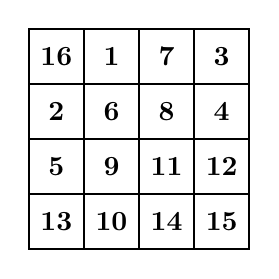
\begin{tikzpicture}[scale=0.7]
    % Disegna la griglia
    \draw[thick] (0,0) rectangle (4,-4);
    \foreach \x in {1,2,3} \draw[thick] (\x,0) -- (\x,-4);
    \foreach \y in {1,2,3} \draw[thick] (0,-\y) -- (4,-\y);

    % Inserisci i numeri
    \node at (0.5,-0.5) {\textbf{16}};
    \node at (1.5,-0.5) {\textbf{1}};
    \node at (2.5,-0.5) {\textbf{7}};
    \node at (3.5,-0.5) {\textbf{3}};
    \node at (0.5,-1.5) {\textbf{2}};
    \node at (1.5,-1.5) {\textbf{6}};
    \node at (2.5,-1.5) {\textbf{8}};
    \node at (3.5,-1.5) {\textbf{4}};
    \node at (0.5,-2.5) {\textbf{5}};
    \node at (1.5,-2.5) {\textbf{9}};
    \node at (2.5,-2.5) {\textbf{11}};
    \node at (3.5,-2.5) {\textbf{12}};
    \node at (0.5,-3.5) {\textbf{13}};
    \node at (1.5,-3.5) {\textbf{10}};
    \node at (2.5,-3.5) {\textbf{14}};
    \node at (3.5,-3.5) {\textbf{15}};
\end{tikzpicture}
\end{minipage}%
\hfill
\begin{minipage}{0.32\textwidth}
\centering
% copia esattamente la stessa struttura con un altro stato se vuoi
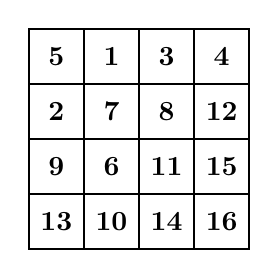
\begin{tikzpicture}[scale=0.7]
    % stessa griglia e contenuto...
        % Disegna la griglia
    \draw[thick] (0,0) rectangle (4,-4);
    \foreach \x in {1,2,3} \draw[thick] (\x,0) -- (\x,-4);
    \foreach \y in {1,2,3} \draw[thick] (0,-\y) -- (4,-\y);

    % Inserisci i numeri
    \node at (0.5,-0.5) {\textbf{5}};
    \node at (1.5,-0.5) {\textbf{1}};
    \node at (2.5,-0.5) {\textbf{3}};
    \node at (3.5,-0.5) {\textbf{4}};
    \node at (0.5,-1.5) {\textbf{2}};
    \node at (1.5,-1.5) {\textbf{7}};
    \node at (2.5,-1.5) {\textbf{8}};
    \node at (3.5,-1.5) {\textbf{12}};
    \node at (0.5,-2.5) {\textbf{9}};
    \node at (1.5,-2.5) {\textbf{6}};
    \node at (2.5,-2.5) {\textbf{11}};
    \node at (3.5,-2.5) {\textbf{15}};
    \node at (0.5,-3.5) {\textbf{13}};
    \node at (1.5,-3.5) {\textbf{10}};
    \node at (2.5,-3.5) {\textbf{14}};
    \node at (3.5,-3.5) {\textbf{16}};
\end{tikzpicture}
\end{minipage}%
\hfill
\begin{minipage}{0.32\textwidth}
\centering
% terzo stato
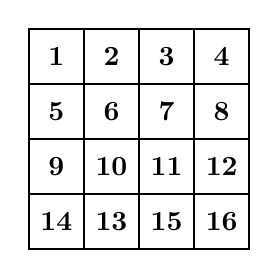
\begin{tikzpicture}[scale=0.7]
    % stessa griglia e contenuto...
        % Disegna la griglia
    \draw[thick] (0,0) rectangle (4,-4);
    \foreach \x in {1,2,3} \draw[thick] (\x,0) -- (\x,-4);
    \foreach \y in {1,2,3} \draw[thick] (0,-\y) -- (4,-\y);

    % Inserisci i numeri
    \node at (0.5,-0.5) {\textbf{1}};
    \node at (1.5,-0.5) {\textbf{2}};
    \node at (2.5,-0.5) {\textbf{3}};
    \node at (3.5,-0.5) {\textbf{4}};
    \node at (0.5,-1.5) {\textbf{5}};
    \node at (1.5,-1.5) {\textbf{6}};
    \node at (2.5,-1.5) {\textbf{7}};
    \node at (3.5,-1.5) {\textbf{8}};
    \node at (0.5,-2.5) {\textbf{9}};
    \node at (1.5,-2.5) {\textbf{10}};
    \node at (2.5,-2.5) {\textbf{11}};
    \node at (3.5,-2.5) {\textbf{12}};
    \node at (0.5,-3.5) {\textbf{14}};
    \node at (1.5,-3.5) {\textbf{13}};
    \node at (2.5,-3.5) {\textbf{15}};
    \node at (3.5,-3.5) {\textbf{16}};
\end{tikzpicture}
\end{minipage}
\caption{Disposizioni esempio usate per misurare i tempo}
\label{fig:esDisp}
\end{figure}

Di cui le prime due configurazioni hanno soluzione mentre la terza non è risolvibile. 

Per confrontare il tutto calcoliamo il tempo impiegato da ASP con il tempo impiegato dal programma scritto in Java che risolve il problema con A*. 
Siccome in ASP dobbiamo specificare il numero di istanti temporali $t$ (numero di mosse) in cui vogliamo risolvere il puzzle, usiamo l'algotimo di A* per trovare una soluzione, ci facciamo comunicare il numero di mosse richieste e impostiamo t a tale valore. 

Il programma A* trova una sequenze di mosse nei seguenti tempi: 
\begin{itemize}
    \item configurazione 1: 25ms e numero di mosse pari a 24; 
    \item configurazione 2: 19ms e numero di mosse pari a 12; 
    \item configurazione 3: 1ms, termina subito;  
\end{itemize}

Il programma ASP trova una sequenza di mosse nei seguenti tempi: 
\begin{itemize}
    \item configurazione 1: 15.22s e numero di mosse pari a 24; 
    \item configurazione 2: 156ms e numero di mosse pari a 12; 
    \item configurazione 3: 150ms (t=10) termina senza trovare una soluzione e indicando che la configurazione fornita non è soddisfacibile; 
\end{itemize}
